%!TEX root = ../thesis.tex
%*******************************************************************************
%****************************** Third Chapter **********************************
%*******************************************************************************
\chapter{PERANCANGAN SISTEM}

% **************************** Define Graphics Path **************************
\ifpdf
    \graphicspath{{Chapter3/Figs/Raster/}{Chapter3/Figs/PDF/}{Chapter3/Figs/}}
\else
    \graphicspath{{Chapter3/Figs/Vector/}{Chapter3/Figs/}}
\fi

Pada bab ini akan dibahas lebih dalam mengenai perancangan tugas akhir yang akan dikerjakan. Gambar~\ref{fig:FlowChart} merupakan diagram alir tahapan pengerjaan proyek akhir yang direncanakan. 

\begin{figure}[ht]
 %\vspace{0.5em}
 \centering
 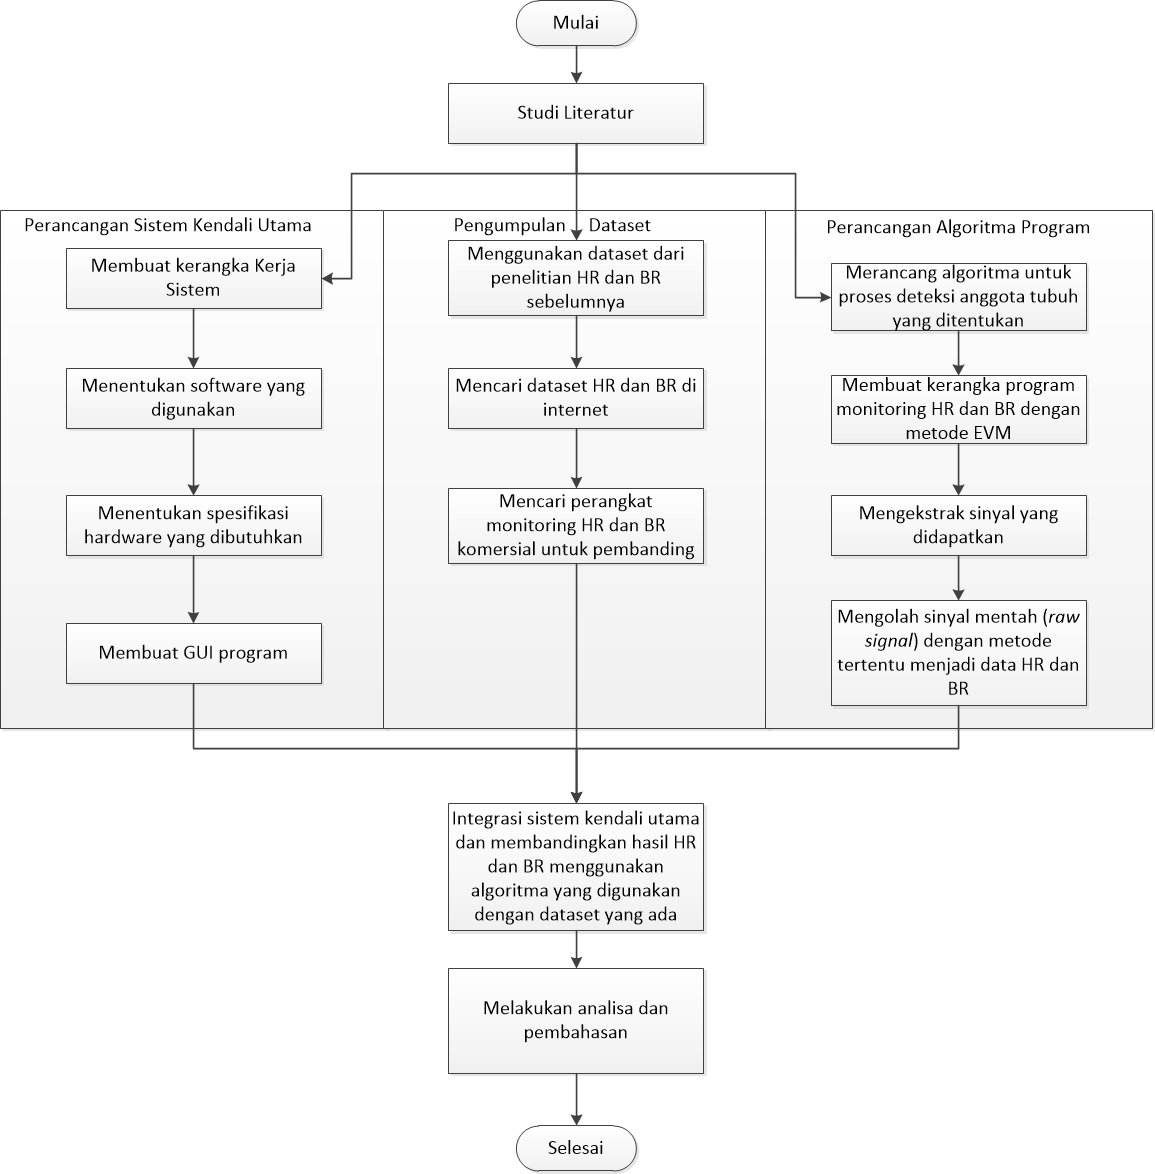
\includegraphics[width=\textwidth]{FlowChart}
 \caption{Diagram Alir Pengerjaan Proyek Akhir}
 \label{fig:FlowChart}   
\end{figure}

\section{Perancangan Sistem Kerja}
Pada bagian ini akan dibahas tentang perancangan sistem yang akan digunakan pada proyek akhir ini. Secara garis besar, proyek akhir ini terdiri atas tiga bagian yaitu mekanisme pendeteksian objek, proses amplifikasi dan ekstraksi sinyal,  dan implementasi pada perangkat sistem benam.


\begin{figure}[ht]
 \vspace{0.5em}
 \centering
 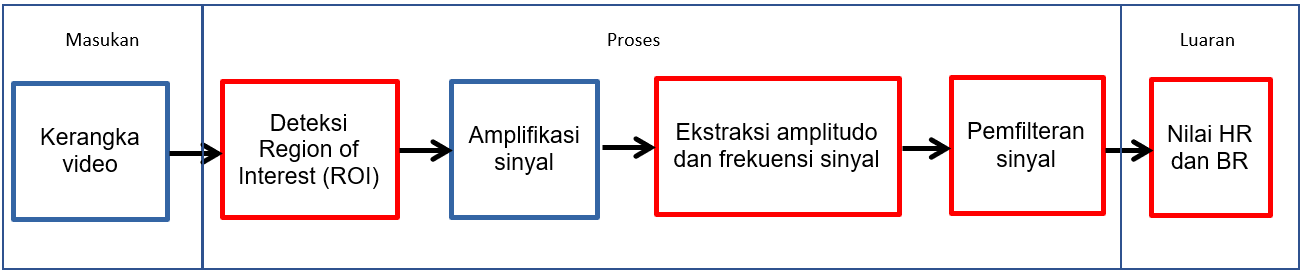
\includegraphics[width=\textwidth]{diagramblok}
 \caption{Perancangan Sistem Kerja}
 \label{fig:diagramblok}   
\end{figure}

Seperti terlihat pada Gambar~\ref{fig:diagramblok}, fokus dari proyek akhir ini ditandai oleh warna merah. Masukan dari proyek akhir ini berupa kerangka video ---diambil menggunakan kamera--- pada bagian tubuh tertentu yang diketahui dapat menunjukkan informasi adanya aktifitas pernapasan maupun sirkulasi darah seperti pada pergelangan tangan, leher, perut dan kepala. Setelah itu kerangka video yang didapat akan diolah pada sistem kendali utama melalui proses pendeteksian area yang menunjukkan adanya perubahan informasi dalam piksel yang berkaitan dengan adanya aktifitas pernapasan maupun sirkulasi darah. Informasi yang berupa sinyal tersebut kemudian akan diamplifikasi dengan menggunakan kerangka dari metode \textit{Eulerian Video Magnification} (EVM) dan akan dilakukan proses ekstraksi ampitudo dan frekuensi dari sinyal tersebut sebagai data mentah untuk diolah lebih lanjut. Proses pengolahan dan pemfilteran sinyal yang merupakan pekerjaan utama dari proyek akhir ini akan dilakukan dengan menggunakan metode yang akan dirancang pada saat pengerjaan proyek akhir. Melalui proses pengolahan data tersebut akan dihasilkan luaran berupa nilai konkret dari HR dan BR yang terdeteksi.

\section{Spesifikasi Hardware}
\subsection{Kamera}
Peran kamera dalam proyek akhir ini sangatlah penting. Kamera merupakan salah satu faktor penting dalam proyek akhir ini karena masukan utama yang digunakan adalah data visual. Pemilihan model kamera yang akan digunakan dapat mempengaruhi kualitas dari video yang ditangkap dan tidak menutup kemungkinan bahwa hal tersebut bisa berdampak pada luaran yang dihasilkan. Semakin besar kapasitas piksel yang dimiliki, maka semakin banyak informasi yang dihasilkan. Namun, hal tersebut dapat mengakibatkan proses pengolahan data menjadi lebih lama. Oleh karena itu, pemilihan model kamera perlu diperhatikan. Pada Tabel \ref{table:spek_cam} disajikan model kamera yang dapat dijadikan opsi dalam pengerjaan proyek akhir ini.

\begin{table}[ht]
\vspace{0.8em}
\caption[Kamera untuk Proses Monitoring HR dan BR]{Contoh Kamera untuk Proses Monitoring HR dan BR}
%\vspace{0.3em}
\centering
\label{table:spek_cam}
\resizebox{.8\textwidth}{!}{%
\begin{tabular}{| c | c |}
\hline 
Model & Spesifikasi \\
\hline
Kinect & Up to 640x480 pixels @30 fps \\
& \textbf{RGB + IR depth-finding}\\
\hline
Netatmo Presence Camera & Up to 1920x1080 pixels \\
& \textbf{RGB + IR}\\
& Deteksi hingga 15 meter\\
& Konektifitas hanya melalui Wifi\\
\hline
Netgear Arlo Q & Up to 1920x1080 pixels HD @30 fps \\
& \textbf{CMOS-RGB + IR}\\
& Deteksi hingga 15 meter\\
& 8x digital zoom\\
\hline
Hikvision Ezviz Mini Plus & Up to 1920x1080 pixels \\
& \textbf{RGB + IR}\\
& Konektifitas hanya melalui Wifi\\
\hline
Logitech 4K Pro Webcam & Up to 4096 x 2160 pixels HD @30 fps \\
& \textbf{RGB + IR}\\
& 5x digital zoom\\
\hline
Logitech C922 Webcam & Up to 1920x1080 pixels HD @30 fps\\
& \textbf{RGB}\\
\hline
Logitech C525 Webcam & Up to 1280 x 720 pixels HD @30 fps\\
& \textbf{RGB}\\
\hline 
\end{tabular} 
}
\end{table}

Kamera kinect memiliki kellebihan dengan adanya teknologi \textit{IR depth-finding} atau yang biasanya dikenal dengan sebutan teknologi RGBd yang dapat memvisualisasikan kedalaman (\textit{depth}) dari suatu obyek. Hal tersebut dapat menjadi suatu kebaruan dalam penelitian mengenai PPG untuk mengetahui pemanfaatan teknologi \textit{IR depth-finding} dalam proses monitoring HR dan BR.

\subsection{ Spesifikasi Perangkat Benam \textit{Embedded Platform}}
Meskipun pengujian algoritma dan sistem menggunakan dilakukan pada \textit{Personal Computer} (PC) atau laptop, namun tujuan dari proyek akhir ini adalah membuat sistem embedded yang digunakan untuk melakukan monitoring HR dan BR yang \textit{non-wearable}. Oleh karena itu, diperlukan perangkat benam yang dapat menjalankan tugas tersebut dengan baik. Hal ini penting mengingat pekerjaan yang dilakukan meliputi pengolahan citra digital serta pengolahan sinyal digital yang memerlukan kecepatan komputasi yang tinggi untuk mendukung keandalan dari sistem. Pengukuran nilai HR dan BR sebisa mungkin dilakukan dalam kondisi \textit{real time} dengan jeda waktu yang singkat mengingat urgensinya. Proses pengolahan citra dan sinyal memerlukan perangkat benam degan CPU dan GPU yang tinggi seperti yang disajikan pada Tabel \ref{table:spek_pc}.

\begin{table}[ht]
\vspace{0.8em}
\caption{Spesifikasi Perangkat Benam untuk Prosas Monitoring HR dan BR}
%\vspace{0.3em}
\centering
\label{table:spek_pc}
\resizebox{\textwidth}{!}{%
\begin{tabular}{| c c |}
\hline 
Model & Spesifikasi \\
\hline
Intel® NUC Kit & Up to 4.20 GHz (4 cores, 8 threads) \\
GPU & \textbf{Up to Radeon™ RX Vega M GH graphics } \\
\hline
Jetson TK1 & NVIDIA "4-Plus-1" 2.32GHz ARM quad-core Cortex-A15 CPU\\
GPU & \textbf{NVIDIA Kepler "GK20a" GPU with 192 SM3.2 CUDA cores (up to 326 GFLOPS)}\\
\hline
Jetson TX1 & Quad ARM® A57/2 MB L2 @1.9 GHz\\
GPU & \textbf{NVIDIA Maxwell ™, 256 CUDA cores}\\
\hline
Jetson TX2 & HMP Dual Denver 2/2 MB L2 @1.4–2.0 GHz + Quad ARM® A57/2 MB L2U @1.2–2.0 GHz \\
GPU & \textbf{NVIDIA Pascal™, 256 CUDA cores}\\
\hline
ODROID-XU4 & Samsung Exynos5422 Cortex™-A15 2Ghz and Cortex™-A7 Octa core CPUs\\
GPU & \textbf{Mali-T628 MP6(OpenGL ES 3.1/2.0/1.1 and OpenCL 1.2 Full profile)}\\
\hline
MintBox 2 & Intel Core i5-3337U dual coreProcessor @1.8GHz (turbo boost up to 2.7GHz)\\
GPU & \textbf{Intel HD Graphics 4000}\\
\hline 
\end{tabular} 
}
\end{table}

Berdasarkan Tabel  \ref{table:spek_pc}, Intel NUC merupakan satu-satunya perangkat yang memiliki kelebihan dalam hal fleksibilitas dikarenakan beberapa komponen dapat dibongkar pasang dan dapat ditingkatkan spesifikasinya sedangkan perangkat lain bersifat tertanam sepenuhnya sehingga memiliki spesifikasi yang tidak dapat diubah.




\section{Perancangan \textit{Graphical User Interface} (GUI)}
Pembuatan \textit{Graphical User Interface} (GUI) bertujan untuk menampilkan proses pengolahan data serta monitoring dan menampilkan data secara \textit{real time} dari kamera yang berfungsi sebagai sensor dalam proses monitoring tingkat HR dan BR pada tubuh. GUI dirancang dengan menggunakan aplikasi matlab yang juga digunakan untuk melakukan proses komputasi dan pengolahan data. Berdasarkan perancangan GUI yang dapat dilihat pada Gambar~\ref{fig:gui}, terdapat dua kotak yang nantinya akan diisi dengan frame video yang akan digunakan untuk menampilkan video masukkan yang dihasilkan dari kamera serta video luaran yang telah diproses. Selain itu, terdapat dua plot diagram yang masing-masing akan digunakan untuk menampilkan data frekuensi dan data amplitudo yang didapatkan selama proses monitoring HR dan BR berlangsung. \textit{Check Box} dapat berisi opsi pengaturan yang dapat digunakan untuk memberikan detil lebih lengkap pada plot diagram yang dibuat. Tombol \textit{Push Button} akan digunakan untuk memulai dan mengakhiri proses monitoring. Pada \textit{Pop-up Menu} dapat digunakan untuk mengubah tampilan yang ada pada GUI.

\begin{figure}[ht]
 \vspace{0.8em}
 \centering
 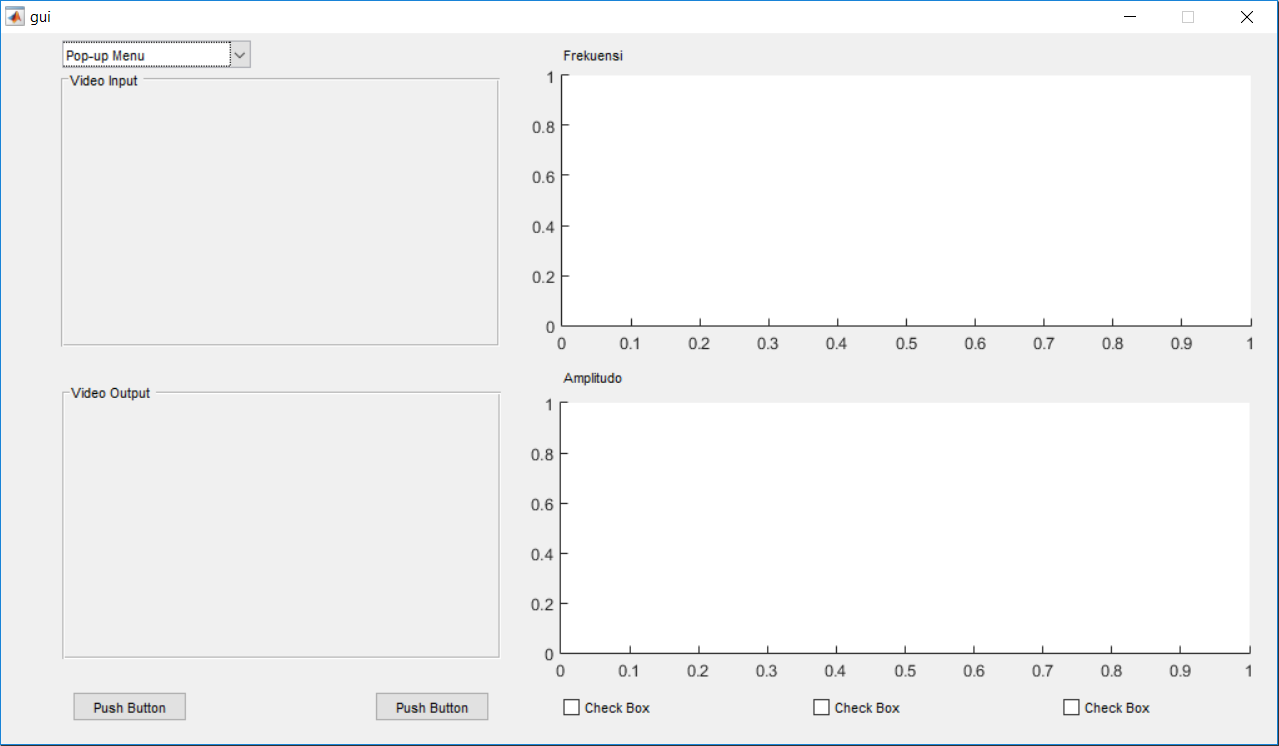
\includegraphics[width=0.8\textwidth]{gui}
 \caption{Rancangan \textit{Graphical User Interface} (GUI)}
 \label{fig:gui}   
\end{figure}

\section{Rencana Validasi Data}
Mengingat bahwa proyek akhir yang akan dikerjakan erat kaitannya dengan bidang kesehatan terlebih menyangkut nyawa seseorang, maka diperlukan proses validasi yang kredibel. Proses validasi data dalam bidang kesahatan paling baik dilakukan dengan cara menjalin kerja sama dengan instansi kesehatan yang berkaitan secara langsung. Namun, dikarenakan proyek akhir ini dibuat untuk penggunaan sehari-hari serta meninjau bahwa prosedur kerja sama dengan instansi kesehatan yang tidak mudah, maka rencana validasi yang realistis dapat dilakukan adalah dengan membandingkan hasil monitoring HR dan BR dengan alat-alat yang memiliki fungsi serupa dan sudah diproduksi dan telah diperjualbelikan secara massal. Pada Tabel \ref{table:alat} disajikan beberapa perangkat \textit{wearable} yang dapat digunakan untuk proses validasi data.

\begin{table}[ht]
\vspace{0.8em}
\caption[Perangkat \textit{Wearable} untuk Pengukuran HR dan BR]{Perangkat \textit{Wearable} komersial untuk Pengukuran HR dan BR}
%\vspace{0.3em}
\centering
\label{table:alat}
\resizebox{.9\textwidth}{!}{%
\begin{tabular}{| c c |}
\hline 
Nama Alat & Keterangan \\
\hline
Pulse Oximeter & Pengukuran HR dan SpO2  \\
 	& Pengukuran pada ujung jari\\
\hline
Fitbit Versa Heart Rate Smart Watch & Pengukuran HR dan kualitas tidur\\
 	& Pengukuran pada pergelangan tangan\\
\hline
Xiaomi Amazfit 2 Smart Watch & Pengukuran HR dan kualitas tidur\\
 	& Pengukuran pada pergelangan tangan\\
\hline
Equivital LifeMonitor & Pengukuran HR dan BR \\
 	& Pengukuran pada wilayah dada\\
\hline
Garmin Strap HRM TRI ANT & Pengukuran HR dan variabilitas HR\\
 	& Pengukuran pada wilayah dada\\
\hline 
\end{tabular} 
}
\end{table}

\section{Perencanaan Jadwal Kerja Penelitian Proyek Akhir}

Pada Tabel \ref{tab:jadwalkerja} di bawah adalah jadwal kerja proyek akhir yang telah disusun dan dibuat berdasarkan metodologi dalam pembuatan sistem monitoring HR dan BR.
\begin{table}[ht]
	\vspace{0.8em}
	\setlength{\arrayrulewidth}{1pt}
	\centering
	\caption{Perencanaan Jadwal Kerja Proyek Akhir}
%	\vspace{0.3em}
	\label{tab:jadwalkerja}
	\resizebox{\textwidth}{!}{%
	\begin{tabular}{|c|l|c|c|c|c|c|c|c|c|c|c|c|c|c|c|}
	\hline
	    & 			& \multicolumn{7}{ c| }{Tahun 2018}	& \multicolumn{7}{ c| }{Tahun 2019}\\\cline{3-16}
	No  &\multicolumn{1}{c|}{Kegiatan}&\multicolumn{7}{ c| }{Bulan}&\multicolumn{7}{ c| }{Bulan}	\\ \cline{3-16}
		& 			&6&7&8&9&10&11&12					&1&2&3&4&5&6&7		\\ \hline
	
	1	& Studi Literatur		&\cellcolor{blue!100}&\cellcolor{blue!100}&\cellcolor{blue!100}&\cellcolor{blue!100}&\cellcolor{blue!100}&\cellcolor{blue!100}&\cellcolor{blue!100}&\cellcolor{blue!100}&\cellcolor{blue!100}&\cellcolor{blue!100}&&&&		\\ \hline
	2	& Koding Program		&&&&\cellcolor{blue!100}&\cellcolor{blue!100}&\cellcolor{blue!100}&\cellcolor{blue!100}&\cellcolor{blue!100}&\cellcolor{blue!100}&\cellcolor{blue!100}&\cellcolor{blue!100}&\cellcolor{blue!100}&\cellcolor{blue!100}&		\\ \hline
	3	& Perancangan Sistem	&&&\cellcolor{blue!100}&\cellcolor{blue!100}&\cellcolor{blue!100}&\cellcolor{blue!100}&\cellcolor{blue!100}&\cellcolor{blue!100}&\cellcolor{blue!100}&\cellcolor{blue!100}&\cellcolor{blue!100}&\cellcolor{blue!100}&\cellcolor{blue!100}&		\\ \hline
	4	& Perancangan Mekanik	& &&&&&\cellcolor{blue!100}&\cellcolor{blue!100}&\cellcolor{blue!100}&\cellcolor{blue!100}&\cellcolor{blue!100}&&&&		\\ \hline
	5	& Perancangan GUI		& &&&&&&\cellcolor{blue!100}&\cellcolor{blue!100}&\cellcolor{blue!100}&\cellcolor{blue!100}&\cellcolor{blue!100}&&&		\\ \hline
	6	& Pengujian Sistem		& &&&&&&\cellcolor{blue!100}&\cellcolor{blue!100}&\cellcolor{blue!100}&\cellcolor{blue!100}&\cellcolor{blue!100}&\cellcolor{blue!100}&\cellcolor{blue!100}&		\\ \hline
	7	& Penyusunan Laporan Akhir	&\cellcolor{blue!100}&\cellcolor{blue!100}&\cellcolor{blue!100}&\cellcolor{blue!100}&\cellcolor{blue!100}&\cellcolor{blue!100}&\cellcolor{blue!100}&\cellcolor{blue!100}&\cellcolor{blue!100}&\cellcolor{blue!100}&\cellcolor{blue!100}&\cellcolor{blue!100}&\cellcolor{blue!100}&\cellcolor{blue!100}		\\ \hline
	\end{tabular}
}
\end{table}

%------------------------------------Template Tabel-----------------------%
%\begin{table}[ht]
%	\vspace{0.5em}
%	\centering
%	\caption{Perencanaan Jadwal Kerja Proyek Akhir}
%	\label{tab:jadwalkerja}
%	\resizebox{\textwidth}{!}{%
%		\begin{tabular}{|c|l|c|c|c|c|c|c|c|c|c|c|c|c|c|c|}
%			\hline
%			& 			& \multicolumn{7}{ c| }{Tahun 2018}	& \multicolumn{7}{ c| }{Tahun 2019}\\\cline{3-16}
%			No  &\multicolumn{1}{c|}{Kegiatan}&\multicolumn{7}{ c| }{Bulan}&\multicolumn{7}{ c| }{Bulan}	\\ \cline{3-16}
%			& 			&6&7&8&9&10&11&12					&1&2&3&4&5&6&7		\\ \hline
%			
%			1	& Studi Literatur		& &&&&&&				&		&&&&&&		\\ \cline{1-16}
%			2	& Koding Program		& &&&&&&				&		&&&&&&		\\ \cline{1-16}
%			3	& Perancangan Sistem	& &&&&&&				&		&&&&&&		\\ \cline{1-16}
%			4	& Perancangan Mekanik	& &&&&&&				&		&&&&&&		\\ \cline{1-16}
%			5	& Perancangan GUI		& &&&&&&				&		&&&&&&		\\ \cline{1-16}
%			6	& Pengujian Sistem		& &&&&&&				&		&&&&&&		\\ \cline{1-16}
%			7	& Penyusunan Laporan Akhir	& &&&&&&				&		&&&&&&		\\ \cline{1-16}
%		\end{tabular}
%	}
%\end{table}